\documentclass[aps,prd,reprint,onecolumn,nofootinbib]{revtex4-2}
\usepackage{amsmath,amssymb,mathrsfs,graphicx,booktabs}
\usepackage[T1]{fontenc}
\begin{document}
\title{Radiation stress under finite observer boosts and
response-preserving energy
moments}
\author{Anonymous research draft}\noaffiliation
\date{27 October 2026}
\begin{abstract}
A low temperature quadrupole approximates radiation stress only within
its amplitude and spectral assumptions. We compare exact bolometric
fourth-power conversion with a linear temperature-to-moment adapter on
the same six positive synthetic skies and the same correlated errors.
Both adapters use the same finite-boost stress residual and invariant
rest-pressure anisotropy. Their physical-target coverage and interval
widths differ even when their method-target calibration is similar.
Separately, energy moments of angular ranks zero, two and four preserve
the complete five-dimensional radiative shear-response operator. In a
retained compression example, rank-four response agreement reaches
numerical precision while a positive angular entropy residual remains.
These are conditional full-sky radiation methods; applying them to
measured channels requires calibrated intensity, spectral completion and
a measured joint error law. The accompanying finite-bandpass foreground
analysis addresses a different inverse problem and does not supply those
inputs.
\end{abstract}\maketitle
\section{Physical moments and two common-input adapters}
Use signature \((-+++ )\), outward sky direction \(n\), photon direction
\(e=-n\), and bolometric energy density per solid angle \(I\) in J
m\(^{-3}\) sr\(^{-1}\). With a calibrated energy temperature, \[
 I=C_\gamma T_E^4,\quad C_\gamma=\frac{\pi k_B^4}{60\hbar^3c^3},\quad
 \rho=\int I\,d\Omega,\quad q=-c\int I n\,d\Omega,\quad
 \pi=\int I\operatorname{STF}(nn)\,d\Omega.
\] The reference temperature is 2.7255 K, giving
\(\rho_{\rm ref}=4.17480092\times10^{-14}\) J/m\(^3\). Set
\(f=q/(c\rho)\), \(P=\pi/\rho\). On the positive moment domain with a
unique timelike Landau eigenbranch, define \[
 \mathscr D=P-\frac{3\operatorname{STF}(ff^T)}{2+\sqrt{4-3|f|^2}},\qquad
 \mathcal A_\gamma=\frac{[\sum_{i=1}^3(p_{L,i}-\rho_L/3)^2]^{1/2}}{\rho_L}.
\] The residual \(\mathscr D\) is an observer-frame STF tensor;
\(\mathcal A_\gamma\) is invariant under observer tetrad changes on this
branch. A zero residual tests a timelike isotropic-pressure rest stress.
It does not require every higher angular multipole to vanish.

The source brightness is
\(I_{\rm rest}/I_{\rm ref}=1+aP_2(n_{{\rm rest},z})\), with
\(a\in\{0,2\times10^{-5},0.02\}\), boosted by
\(\boldsymbol\beta=b(0.6,0,0.8)\), \(b\in\{0.00123,0.3\}\). The complete
positive temperature sky is obtained from this specified boost,
retaining its higher modes. The analytic target is the Lorentz transform
of \(\operatorname{diag}(1,1/3-a/15,1/3-a/15,1/3+2a/15)\rho_{\rm ref}\),
so \(\mathcal A_{\gamma,\rm true}=\sqrt6|a|/15\).

Only the three temperature dipole and five temperature STF coordinates
are perturbed. Their Gaussian standard deviations are
\(7.5\times10^{-6}\) and \(9.375\times10^{-7}\), and their correlation
is \(0.8I_8+0.2ss^T\), \(s=(1,-1,1,1,-1,1,-1,1)\). Monopole and higher
temperature modes are noiseless known inputs. Both methods receive
identical errors. The exact adapter integrates the fourth power of that
sky. The linear adapter uses \(f_{\rm lin}=-4d_T/3\) and
\(P_{\rm lin}=8Q_T/15\), with the same monopole normalization, then
applies the same exact \(\mathscr D\) and Landau readout. This isolates
the temperature-to-moment approximation. The joint flux/stress
covariance, including its three-by-five cross block, is retained; it is
not replaced by independent dipole and quadrupole errors.
\section{Conditional calibration, coverage and widths}
Each case uses 8,191 calibration skies and 4,096 disjoint test skies.
Calibration is pointwise around the known noiseless response of each
method. For \(\mathscr D\), the confidence-region radius is the 7,783rd
ordered calibration norm error, producing a five-dimensional ball. For
\(\mathcal A_\gamma\), the interval subtracts the 7,988th and 204th
ordered calibration errors and intersects the result with
\([0,\infty)\). An upper endpoint below zero produces an empty interval
and is counted as noncoverage. The exact physical target and the
noiseless method target are assessed separately; no bias correction is
fitted to force them to coincide.

\begin{table}[htbp]
\centering\small
\caption{Physical-target hit counts and finite-test 95-percent Clopper--Pearson intervals. $N=4096$ for every row. Calibration uses 8191 separate draws; calibration-content uncertainty is distinct from these test intervals.}\label{tab:radcoverage}
\begin{tabular}{llll}
\toprule
Case & Method & $\mathscr D$ hits/N [interval] & $\mathcal A_\gamma$ hits/N [interval] \\
\midrule
a0\_b0.00123 & exact & 3872/4096 [0.9379,0.9521] & 3914/4096 [0.9488,0.9617] \\
a0\_b0.00123 & linear & 3035/4096 [0.7273,0.7543] & 1545/4096 [0.3623,0.3922] \\
a0\_b0.3 & exact & 3934/4096 [0.9540,0.9662] & 3907/4096 [0.9470,0.9601] \\
a0\_b0.3 & linear & 0/4096 [0.0000,0.0009] & 0/4096 [0.0000,0.0009] \\
a2e-05\_b0.00123 & exact & 3890/4096 [0.9426,0.9562] & 3862/4096 [0.9353,0.9498] \\
a2e-05\_b0.00123 & linear & 3055/4096 [0.7322,0.7591] & 3654/4096 [0.8822,0.9014] \\
a2e-05\_b0.3 & exact & 3919/4096 [0.9501,0.9628] & 3892/4096 [0.9431,0.9567] \\
a2e-05\_b0.3 & linear & 0/4096 [0.0000,0.0009] & 0/4096 [0.0000,0.0009] \\
a0.02\_b0.00123 & exact & 3888/4096 [0.9420,0.9557] & 3905/4096 [0.9465,0.9596] \\
a0.02\_b0.00123 & linear & 0/4096 [0.0000,0.0009] & 0/4096 [0.0000,0.0009] \\
a0.02\_b0.3 & exact & 3873/4096 [0.9382,0.9523] & 3901/4096 [0.9454,0.9587] \\
a0.02\_b0.3 & linear & 0/4096 [0.0000,0.0009] & 0/4096 [0.0000,0.0009] \\
\bottomrule
\end{tabular}
\end{table}

\begin{table}[htbp]
\centering\small
\caption{Dimensionless widths displayed in units of $10^{-6}$. Empty scalar intervals count as noncoverage; only the explicitly counted nonempty intervals enter their mean.}\label{tab:radwidth}
\begin{tabular}{llllll}
\toprule
Case & Method & Ball diameter $/10^{-6}$ & Empty fraction & $N_{\rm nonempty}$ & Mean width $/10^{-6}$ \\
\midrule
a0\_b0.00123 & exact & 3.390224 & 0.021729 & 4007 & 0.638565 \\
a0\_b0.00123 & linear & 3.380536 & 0.000000 & 4096 & 1.490733 \\
a0\_b0.3 & exact & 8.369104 & 0.029053 & 3977 & 1.884719 \\
a0\_b0.3 & linear & 27.694794 & 0.000000 & 4096 & 33.419948 \\
a2e-05\_b0.00123 & exact & 3.396305 & 0.000000 & 4096 & 1.887453 \\
a2e-05\_b0.00123 & linear & 3.388694 & 0.000000 & 4096 & 1.932102 \\
a2e-05\_b0.3 & exact & 8.454129 & 0.000000 & 4096 & 5.066372 \\
a2e-05\_b0.3 & linear & 27.748430 & 0.000000 & 4096 & 33.723377 \\
a0.02\_b0.00123 & exact & 3.415737 & 0.000000 & 4096 & 1.990204 \\
a0.02\_b0.00123 & linear & 3.420747 & 0.000000 & 4096 & 1.995023 \\
a0.02\_b0.3 & exact & 8.441110 & 0.000000 & 4096 & 6.450267 \\
a0.02\_b0.3 & linear & 27.647888 & 0.000000 & 4096 & 33.857972 \\
\bottomrule
\end{tabular}
\end{table}

For the pure-boost case at \(b=0.00123\), the exact and linear
physical-target \(\mathscr D\) counts are 3,872/4,096 and 3,035/4,096,
while the invariant-anisotropy counts are 3,914/4,096 and 1,545/4,096.
Their \(\mathscr D\) ball diameters are nearly equal,
\(3.390\times10^{-6}\) and \(3.381\times10^{-6}\). Thus similar widths
can conceal different target bias. The linear method-target coverage
remains near its nominal level across the cases even where its
physical-target coverage fails.

At \(a=0,b=0.3\), the exact \(\mathscr D\) count is 3,934/4,096, or
0.960449, with a retained 95-percent interval {[}0.954021,\allowbreak 0.966209{]}.
This single high estimate is an unadjusted finite-simulation diagnostic
among the reported comparisons, not a claim of exact 95-percent
coverage. Calibration-content uncertainty is separate: under continuous
errors its retained central intervals are {[}0.945254,\allowbreak 0.954684{]} for
the ball and {[}0.945382,\allowbreak 0.954801{]} for the scalar interval. No seeds,
quantiles or sample counts were adjusted. Empty exact-method scalar
intervals occur in 89 and 119 test skies in the two pure-boost cases;
corresponding nonempty means use 4,007 and 3,977 skies. Empirical
measured-sky error-law misspecification is outside these intervals.

\begin{figure}[htbp]
\centering
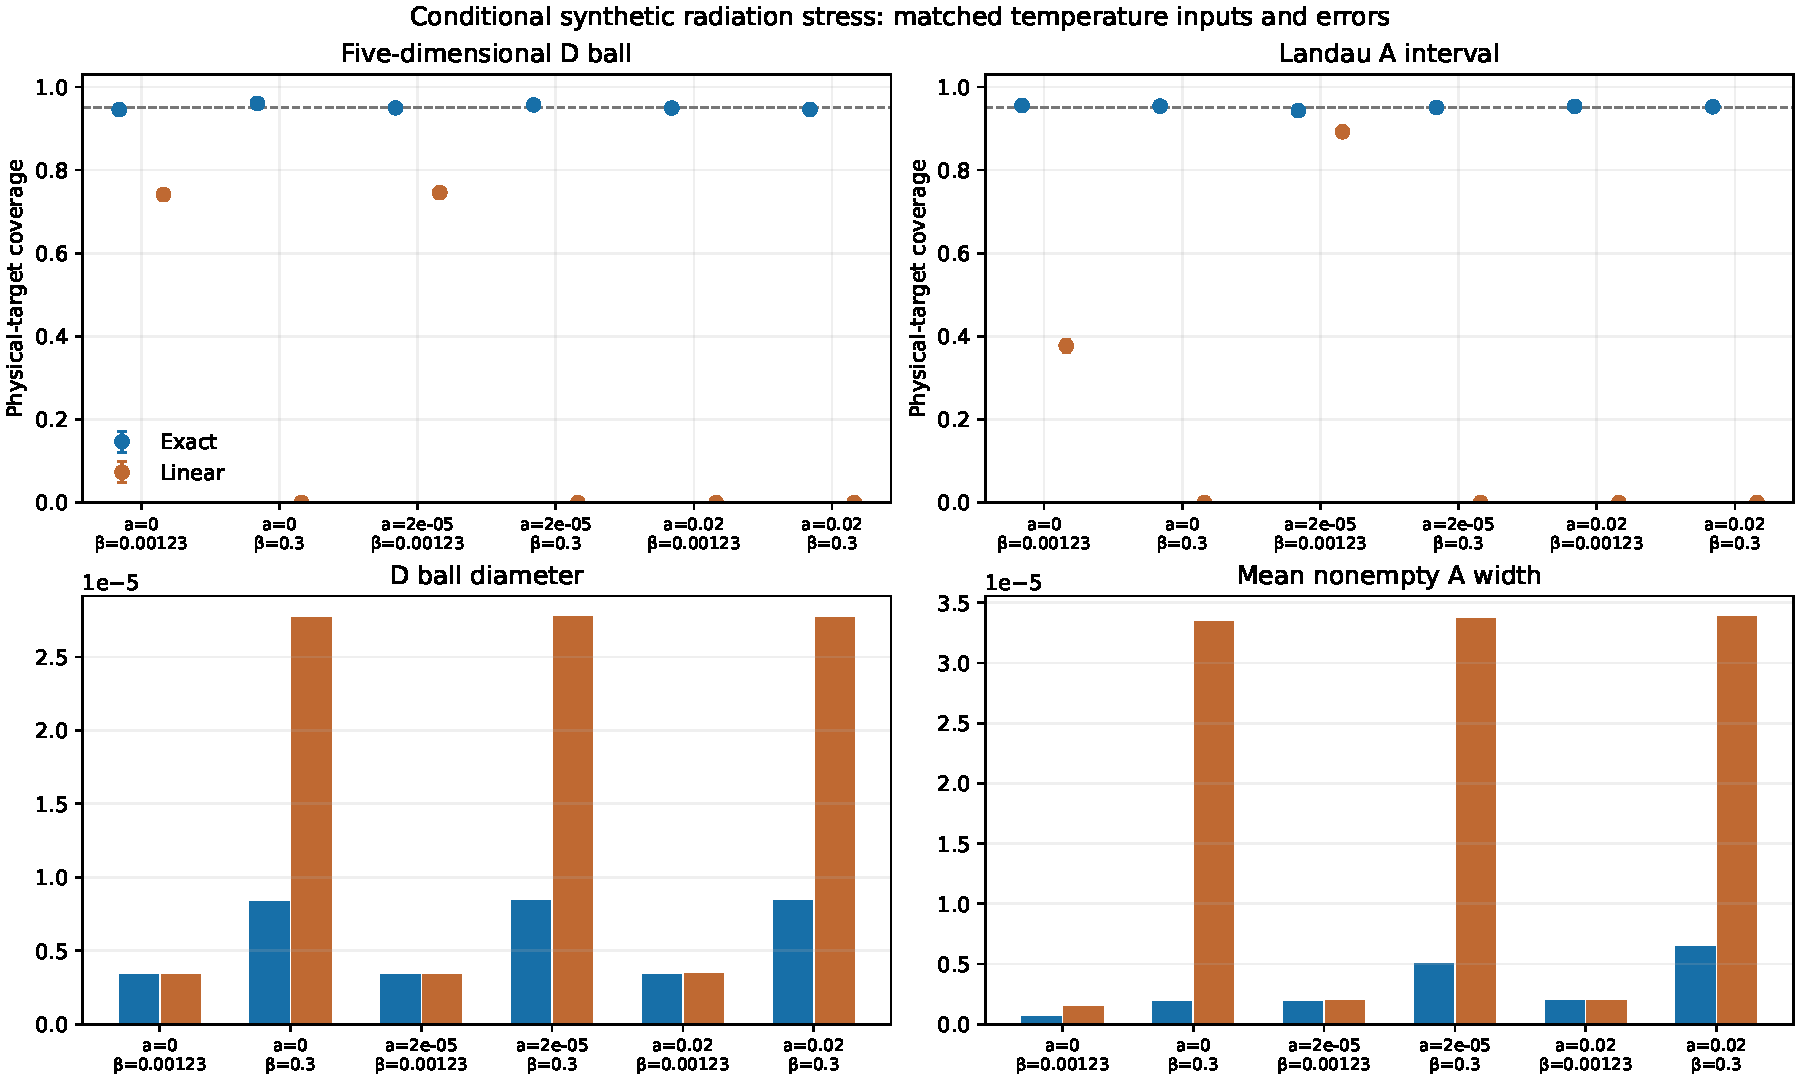
\includegraphics[width=0.95\linewidth]{comparison.pdf}
\caption{Common-input synthetic comparison of exact and linear temperature adapters. Upper panels show physical-target coverage and finite-test Clopper--Pearson intervals; the dashed line is the nominal calibration level. Lower panels show the five-dimensional residual-ball diameter and the mean width of nonempty rest-anisotropy intervals. Empty intervals count as noncoverage and are excluded only from the explicitly labeled nonempty width means. Both methods use the same correlated temperature errors, with noiseless known monopole and higher modes. These are pointwise oracle benchmarks, not calibrated intervals for an unknown observed CMB sky.}
\end{figure}
\section{The moments needed for the target response}
Let \(H_4=\int I(e)e_{\langle i}e_je_ke_{l\rangle}\,d\Omega\). On the
five-dimensional STF space, the instantaneous radiative response is \[
 \mathcal L_I S=\frac{8\rho}{15}S+
 \frac{10}{7}\operatorname{STF}[\tfrac12(S\pi+\pi S)]-H_4:S,
\] with quadratic form \[
 S:\mathcal L_I S=\int I(e)[2|Se|^2-(e^TSe)^2]\,d\Omega.
\] Only energy moments of ranks zero, two and four enter. Matching these
moments therefore preserves the entire operator, independently of
unresolved higher angular structure. In the retained compression
experiment, the operator error normalized by \(\rho_0\) is 0.00654243536
at rank two and \(3.3393\times10^{-16}\) at rank four on the primary
quadrature, while the positive normalized angular entropy residual is
\(9.37160903\times10^{-5}\). The higher quadrature gives rank-four error
\(4.3301\times10^{-15}\); the conclusion is numerical agreement at the
checked precision, not exact binary equality.

\begin{table}[htbp]
\centering\small
\caption{Both retained angular quadratures and response errors normalized by $\rho_0$; entropy residuals use the isotropic entropy normalization.}\label{tab:radresponse}
\begin{tabular}{llll}
\toprule
Quadrature & Rank & Operator error & Entropy residual \\
\midrule
256 & 2 & 0.0065424354 & 0.00037370961 \\
256 & 4 & 3.3393191e-16 & 9.371609e-05 \\
320 & 2 & 0.0065424354 & 0.00037370961 \\
320 & 4 & 4.3301414e-15 & 9.371609e-05 \\
\bottomrule
\end{tabular}
\end{table}

\begin{table}[htbp]
\centering\small
\caption{All five rank-four response eigenvalues divided by $\rho_0$. Full matrices accompany the numerical supplement.}\label{tab:radeigen}
\begin{tabular}{llllll}
\toprule
Quadrature & $\lambda_1$ & $\lambda_2$ & $\lambda_3$ & $\lambda_4$ & $\lambda_5$ \\
\midrule
256 & 0.5034920635 & 0.5034920635 & 0.5526984127 & 0.5526984127 & 0.5542857143 \\
320 & 0.5034920635 & 0.5034920635 & 0.5526984127 & 0.5526984127 & 0.5542857143 \\
\bottomrule
\end{tabular}
\end{table}

For the positive \(e^{8\mu^2}\) brightness family, a sufficient entropy
lower bound is \(-0.352935\rho\), while the actual minimum response
eigenvalue is \(0.12823282\rho>0\). A failed sufficient certificate does
not establish loss of coercivity; the finite operator spectrum provides
the direct check. If a specified transport branch supplies
\(\mathcal L_I\sigma=-R\), a shear estimate also needs the derivative
residual \(R\), its frame and its error. That residual is absent here,
so no matter shear is inferred from instantaneous brightness alone.

The finite-bandpass foreground problem and this bolometric calculation
constrain different objects. A calibrated intensity/spectral completion
is needed to carry measured channel amplitudes into the positive energy
moments used above. Polarization E is not such an intensity, and
evaluating number and energy from one imposed blackbody temperature does
not create a second independent observed channel. The present
contribution is a response-specific stopping criterion and a
matched-input stress comparison under a stated synthetic law.

\begin{thebibliography}{1}
\bibitem{source} The source-bound numerical supplement distributed with this manuscript retains the complete moment matrices, common-input comparison statistics and qualification limitations.
\end{thebibliography}\end{document}
